% !TEX TS-program = xelatex
% !TEX encoding = UTF-8 Unicode
% !Mode:: "TeX:UTF-8"

\documentclass{resume}
\usepackage{graphicx}
\usepackage{tabu}
\usepackage{tabularx, booktabs}
\usepackage{multirow}
\usepackage{makecell}
\usepackage{zh_CN-Adobefonts_external} % Simplified Chinese Support using external fonts (./fonts/zh_CN-Adobe/)
% \usepackage{NotoSansSC_external}
% \usepackage{NotoSerifCJKsc_external}
% \usepackage{zh_CN-Adobefonts_internal} % Simplified Chinese Support using system fonts
\usepackage{linespacing_fix} % disable extra space before next section
\usepackage{cite}

\begin{document}
\pagenumbering{gobble} % suppress displaying page number

\renewcommand\arraystretch{1.5}
\begin{tabular}{p{13cm} p{4cm}}
  \textbf{\huge 林祎凡} & \multirowcell{4}{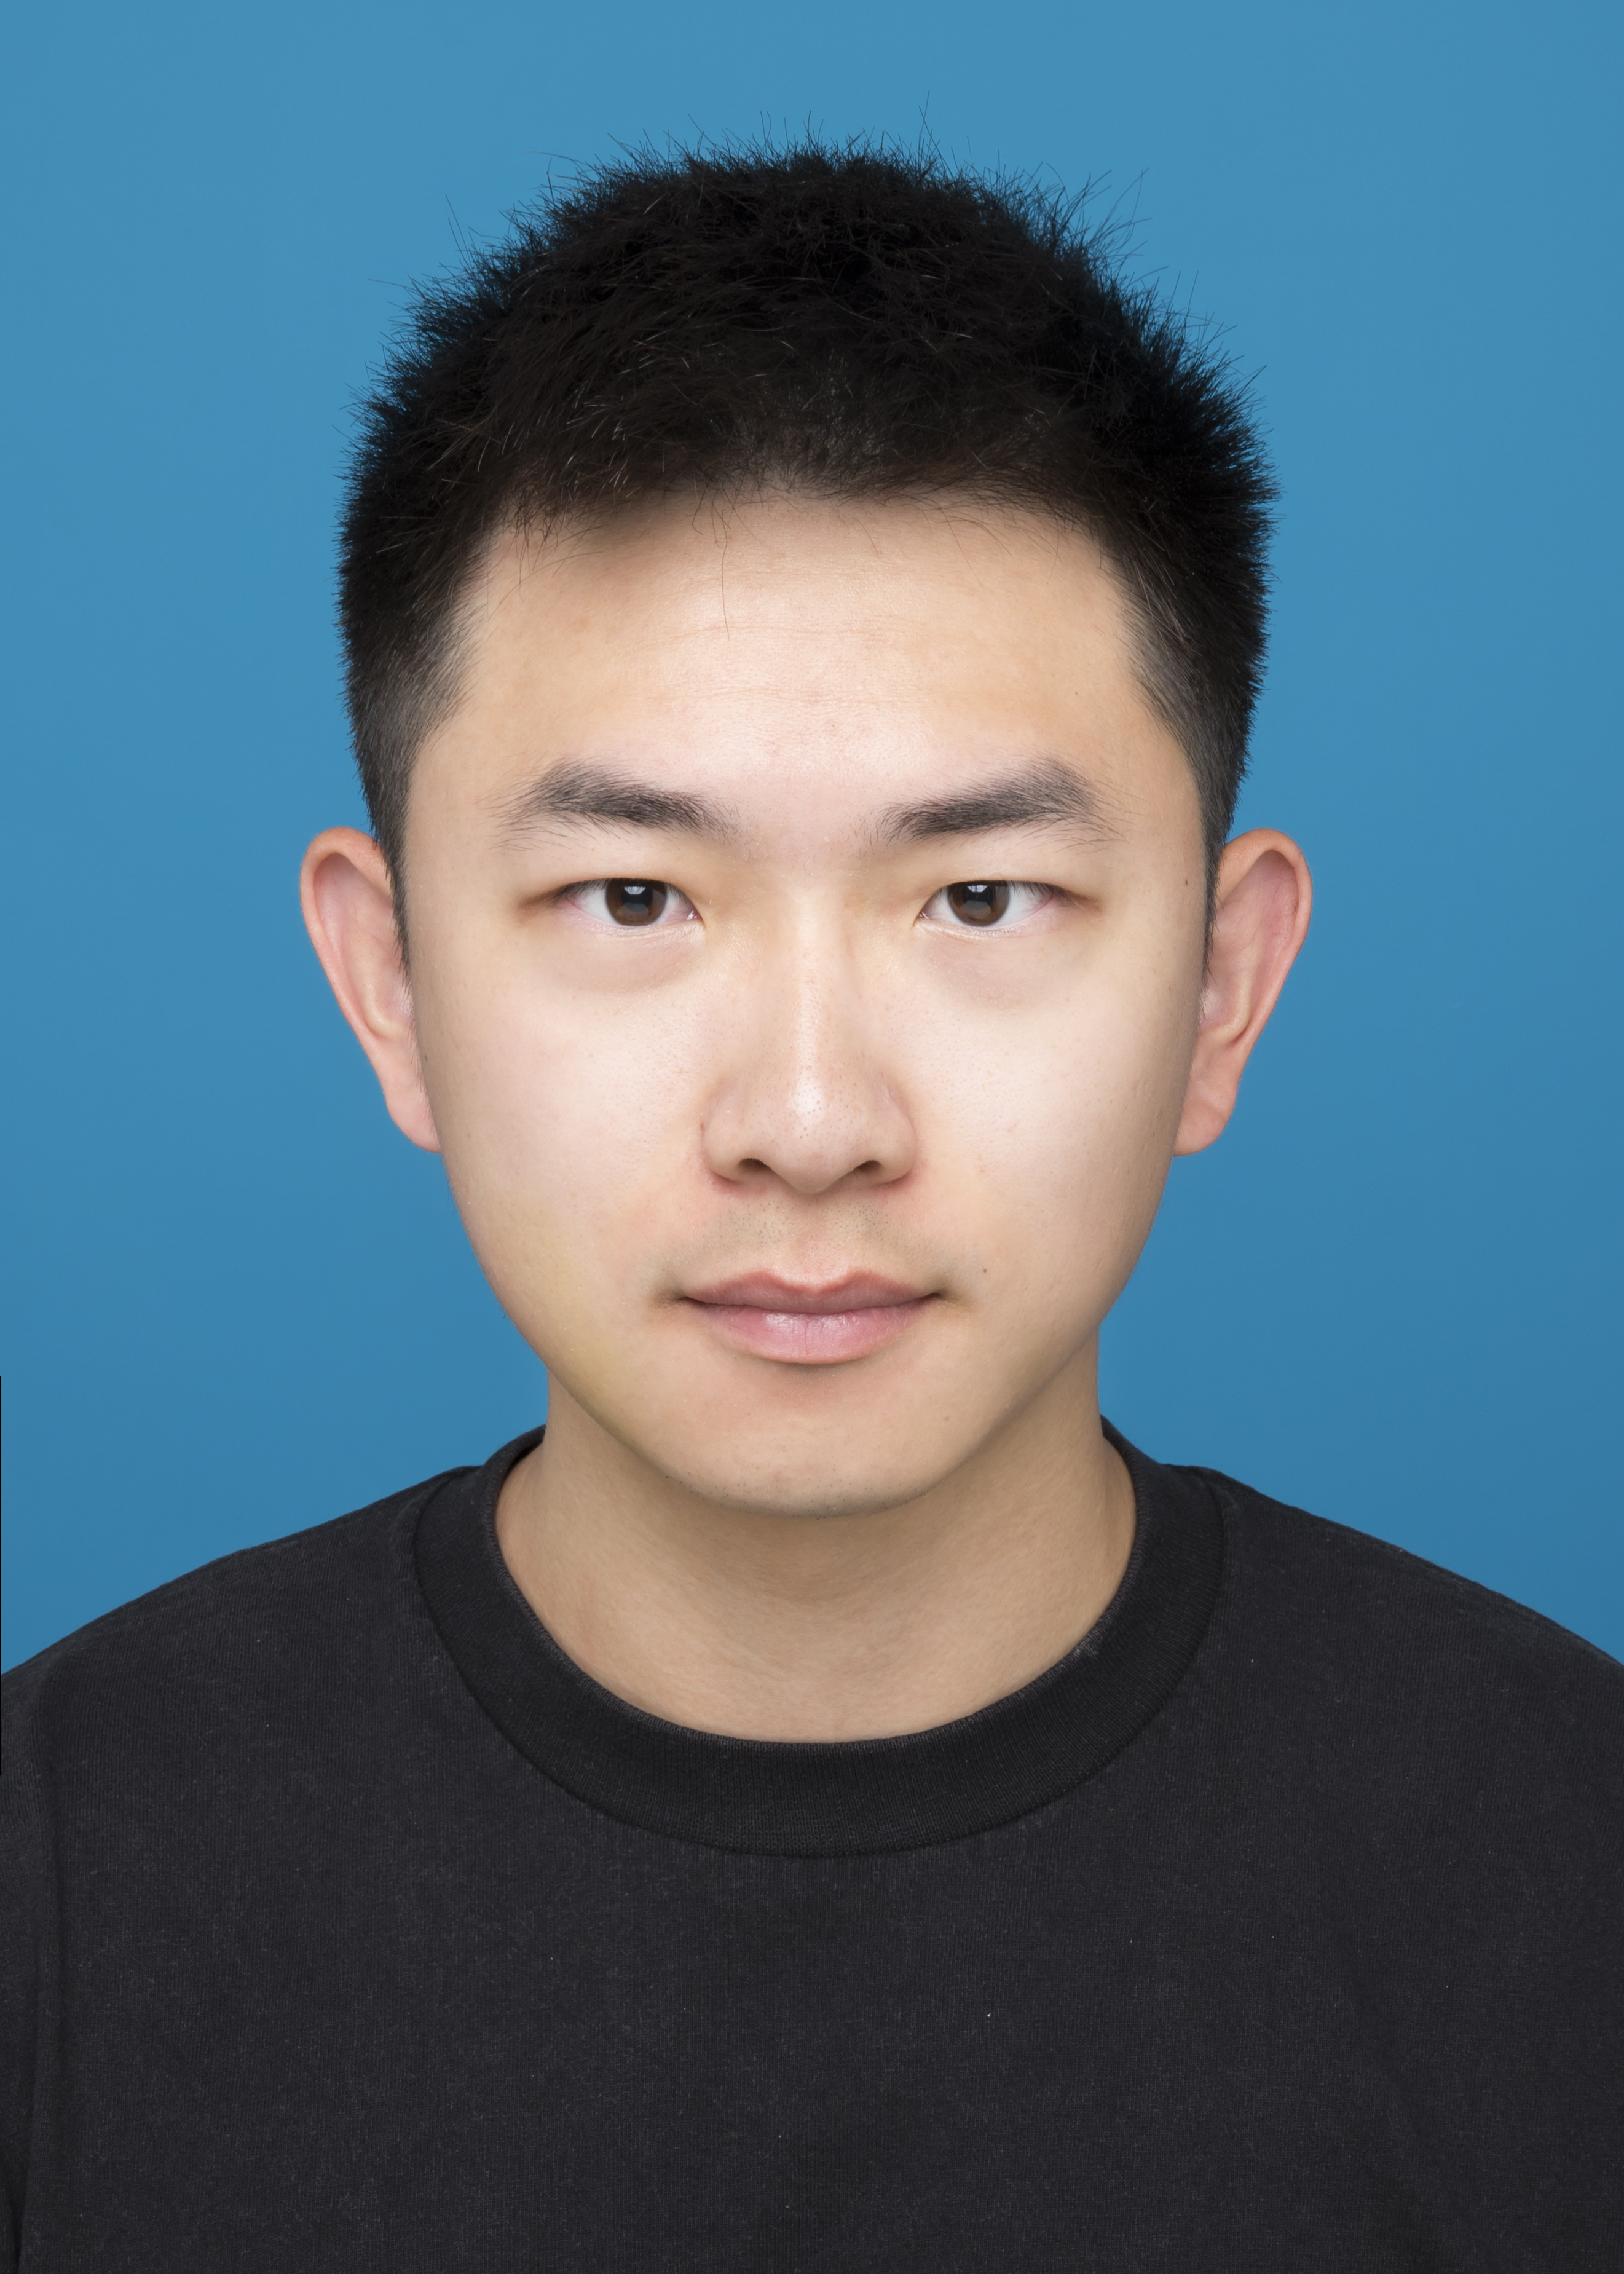
\includegraphics[scale=0.5]{avatar}} \\
  \email{yifanlin@mail.ustc.edu.cn} & \\
  \phone{(+86) 158-5519-0679} & \\
\end{tabular}


% \name{方缙}

% \basicInfo{
%   \email{fangjin98@mail.ustc.edu.cn} \textperiodcentered\ 
%   \phone{(+86) 181-5566-1676} \textperiodcentered\ 
%   \homepage[www.fangjin.site]{www.fangjin.site}
% }

\section{教育背景}

\datedsubsection{\textbf{中国科学技术大学} \quad \textit{硕博连读} \quad 计算机科学与技术}{2022.9-2027.6 (预计)}
\begin{itemize}
  \item 研究方向: 数据中心网络、可编程网络、分布式训练
  \item 导师:徐宏力、赵功名
\end{itemize}

\datedsubsection{\textbf{中国科学技术大学} \quad \textit{学士} \qquad \quad 少年班学院}{2018.9-2022.6}

\section{项目经历}

\datedsubsection{\textbf{面向 AI 流量的高性能路由与调度}}{华为2012网络技术实验室}
\datedsubsection{\textit{技术点负责人}}{2024.6-2024.9}
\begin{itemize}[parsep=0.5ex]
  \item 在AI大模型训练集群中,网络通信已成为限制训练速度的关键瓶颈,优化网络通信至关重要
  \item 调研现有的AI集群时序控制方案,发现其难以处理华为AI集群内的复杂时序控制问题,据此提出了新的时序控制方案,可以有效解决已有方案的不足之处
\end{itemize}

\datedsubsection{\textbf{东数西算背景下任务全域调度研究}}{华为2012网络技术实验室}
\datedsubsection{\textit{算法设计、系统开发}}{2023.5-2024.5}
\begin{itemize}[parsep=0.5ex]
  \item 调研发现在“东数西算”战略背景下,现有任务调度方案效率低下,难以进行全域任务调度。据此通过分析华为现网SKU资源需求、区域资源成本、区域服务质量等指标提出了基于子图匹配的高效任务调度算法,该算法在最优性和时间效率方面都得到了理论保障
  \item 构建了基于 Java 的全域调度算法仿真系统,该系统支持高达 1000 个地理区域的任务调度规模,并确保单次调度时间不超过 300 毫秒。在仿真平台进行的实验表明,算法
  \item 撰写名为“RAISE: A Recommendation Framework for Service Placement in Geo-distributed Clouds” 的论
  文并投稿CCF A类会议INFOCOM'24
\end{itemize}

\section{科研经历}

\datedsubsection{\textbf{基于可编程网络实现精准模拟网络故障}}{中科大苏高院,苏州}
\datedsubsection{\textit{系统开发}}{2022.12-2023.4}
\begin{itemize}[parsep=0.5ex]
  \item 调研发现基于端主机的故障注入难以覆盖大量复杂网络故障场景,据此提出利用可编程交换机来进行故障注入
  \item 设计并实现了用户友好的多后端故障注入系统,提供一系列参数供用户自定义流量协议,并在多个流行的分布式系统任务中测试该系统并验证故障注入效果
\end{itemize}

\datedsubsection{\textbf{网内聚合场景下可编程交换机的部署问题}}{之江实验室,杭州}
\datedsubsection{\textit{算法设计}}{2022.6-2022.9}
\begin{itemize}[parsep=0.5ex]
  \item 调研发现网内聚合场景下可编程交换机的部署成本高,据此提出了基于斯坦纳树问题的可编程交换机增量部署算法,算法的性能得到了理论保障
  \item 经过实验评估,该算法可以在不影响训练性能的前提下节约60\%的可编程交换机数量
\end{itemize}

\section{学术成果}

\begin{enumerate}[parsep=0.5ex]
  \item \textbf{Y. Lin}, G. Zhao, J. Wen, L. Luo, C. Huang, \textit{RAISE: A Recommendation Framework for Service Placement in Geo-distributed Clouds}, INFOCOM'25 在投
  \item 赵功名, 吴昌博, 徐宏力, 包剑峰, 方缙, \textbf{林祎凡}, 黄河, 黄刘生, \textit{基于网内聚合的分布式模型训练加速
  综述}, 计算机研究与发展, 在投
\end{enumerate}

\section{奖项荣誉}

\begin{itemize}[parsep=0.5ex]
  \item \datedline{2022 英特尔 P4 中国黑客松 \textbf{The Exellent Prize}}{}
  \item \datedline{中国科学技术大学硕士研究生一等学业奖学金}{}
\end{itemize}

\end{document}
